\section{Experiment Score}
\label{sec:experiment}

This section presents the experimental results validating our implementation, structured into two main parts: demonstration of iterative decoding and reporting of the best FID scores obtained.

\subsection{Iterative Decoding}
In this part, we demonstrate the iterative decoding process for different mask scheduling strategies.

\subsubsection{Mask in Latent Domain}
Present visualizations of the mask distribution over iterations using different scheduling strategies (cosine, linear, square).

\begin{figure}[H]
    \centering
    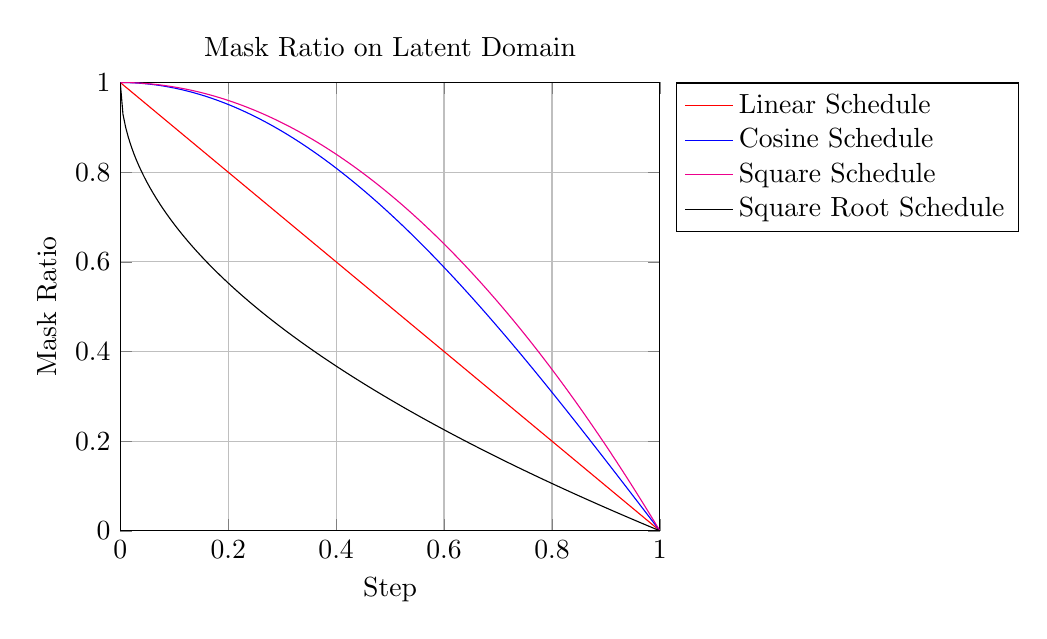
\begin{tikzpicture}
        \begin{axis}[
                % width=0.4\linewidth,
                % height=0.4\linewidth,
                grid=major,
                title={Mask Ratio on Latent Domain},
                legend pos=outer north east,
                legend cell align=left,
                xmin=0,xmax=1,
                ymin=0,ymax=1,
                xlabel={Step},
                ylabel={Mask Ratio},
            ]
            \addplot[domain=0:1,samples=200,red]{1-x};
            \addlegendentry{Linear Schedule}
            \addplot[domain=0:1,samples=200,blue]{(cos(deg(x)*pi/2))};
            \addlegendentry{Cosine Schedule}
            \addplot[domain=0:1,samples=200,magenta]{1-x^2};
            \addlegendentry{Square Schedule}
            \addplot[domain=0:1,samples=200,black]{(1-sqrt(x))};
            \addlegendentry{Square Root Schedule}
        \end{axis}
    \end{tikzpicture}
\end{figure}

\textbf{Cosine Schedule:}

\textit{[Insert visualization here]}

\textbf{Linear Schedule:}

\textit{[Insert visualization here]}

\textbf{Square Schedule:}

\textit{[Insert visualization here]}

\subsubsection{Predicted Images}
Show the intermediate predicted images at different decoding iterations using the scheduling strategies.

\textbf{Cosine Schedule:}

\textit{[Insert predicted images here]}

\textbf{Linear Schedule:}

\textit{[Insert predicted images here]}

\textbf{Square Schedule:}

\textit{[Insert predicted images here]}

\subsection{Best FID Score}

\subsubsection{Results}
Report the best FID scores obtained under each mask scheduling strategy.

\begin{itemize}
    \item \textbf{Cosine Schedule:} \textit{[FID Score]}
    \item \textbf{Linear Schedule:} \textit{[FID Score]}
    \item \textbf{Square Schedule:} \textit{[FID Score]}
\end{itemize}

\subsubsection{Experimental Settings}
Provide the specific hyperparameter settings and training strategies that yielded the best FID scores:

\begin{itemize}
    \item \textbf{Learning Rate:} $1\times10^{-4}$
    \item \textbf{Batch Size:} $8$
    \item \textbf{Epochs:} $100$
    \item \textbf{Sweet Spot:} $8$
    \item \textbf{Total Iterations:} $12$
\end{itemize}
